%%---%% Physics Lab Report Version 0.6 - 1.febrúar 2023 %%---%%
% Höfundur/Author: Hákon Örn Árnason - hakona07 AT ru.is
% Viðhaldið af/Maintained by: Hákon Örn Árnason - hakona07 AT ru.is
%%%%%%%%%%%%%%%%%%%%%%%%%%%%%%%%%%%%%%%%%%%%%%%%%%%%%%%%%%%
% Credits to:
% Math template by Hlynur Arnarsson
% How to write text by Andrei Manolescu, Haraldur Auðunsson, Sigurður Ingi Erlingsson, version 050918
% Hákon Valur Haraldsson - figures and tables additions.
%%%%%%%%%%%%%%%%%%%%%%%%%%%%%%%%%%%%%%%%%%%%%%%%%%%%%%%%%%%

\documentclass{scrartcl}
% Skapalón frá Hlyni Arnórssyni
% Physics Version 0.2 - 10.Jan 2020
% ---------- Blaðsíðustillingar ---------- 
\usepackage{geometry}

\geometry{
	paper=a4paper, % letterpaper lika til
	top=2.5cm, % Top margin
	bottom=1cm, % Bottom margin
	left=2.5cm, % Left margin
	right=2.4cm, % Right margin
	headheight=0.75cm, % Header height
	footskip=1.5cm, % Space from the bottom margin to the baseline of the footer
	headsep=0.75cm, % Space from the top margin to the baseline of the header
	%showframe, % Uncomment to show how the type block is set on the page
}

% ---------- Íslenska ---------- 
\usepackage[T1]{fontenc}
\usepackage[utf8]{inputenc}
\usepackage[icelandic]{babel} % Setið 'english' í hornklofana ef skýrslan er alfarið á ensku.

% ---------- Stærðfræðipakkar frá AMS ---------- 

\usepackage{amsmath, amsfonts, amsthm, amssymb} % Stærðfræðipakkar
\usepackage{braket, nicefrac} % fyrir mengi, brotabrot

% ---------- Fyrir SI Einingar ---------- 
\usepackage{siunitx}

% ---------- Listar/ númeringar ---------- 
\usepackage{enumitem, multicol}

% ---------- Fyrir innsetningu mynda ---------- 
\usepackage{graphicx, float} 
\usepackage{keystroke}

% ---------- Til að teikna/tekka myndir ---------- 
\usepackage{tikz}
\usepackage{tkz-euclide}
\usetikzlibrary{math}
\usepackage{fourier}
\usetikzlibrary{quotes,angles}
\usepackage{tkz-euclide}
\usetikzlibrary{calc}
\usepackage[siunitx, nooldvoltagedirection]{circuitikz} %%<--- Circuit Diagrams/Rafrása myndir
\usepackage{csquotes}
%%%%%%%%%%%%%%%%%%%%%%%%%% Hyperlink References %%%%%%%%%%%%%%%%%%%%%%%%%%%
\usepackage[colorlinks=true, linkcolor=blue, citecolor=blue, urlcolor=blue, bookmarks=true, breaklinks=true]{hyperref}
\labelformat{equation}{(#1)} %jöfnu fix
\def\equationautorefname#1{}%for autoref, gobble the space
%%%%%%%%%%%%%%%%%%%%%%%%%%
% ---------- Nýtt Matlab viðmót ---------- 
\usepackage{listings}
\usepackage{fancyvrb}

\def\lstbasicfont{\fontfamily{pcr}\selectfont\normalsize}
\definecolor{mygreen}{RGB}{28,172,0} 
\definecolor{mylilas}{RGB}{170,55,241}
\lstset{language=Matlab,%
	basicstyle={\lstbasicfont},
	breaklines=true,%
	morekeywords={matlab2tikz},
	keywordstyle=\color{blue},%
	morekeywords=[2]{1}, keywordstyle=[2]{\color{black}},
	identifierstyle=\color{black},%
	stringstyle=\color{mylilas},
	commentstyle=\color{mygreen},%
	showstringspaces=false, %without this there will be a symbol in the places where there is a space
	numbers=left,%
	numberstyle={\tiny \color{black}},% size of the numbers
	numbersep=5 pt, % this defines how far the numbers are from the text 
	inputencoding=latin1,
	backgroundcolor = \color{gray!3},
	framexleftmargin= -1 mm,
	frame=none,
	rulesepcolor=\color{blue!30},
	extendedchars=true,
	emph={logical},emphstyle=\color{blue},	
	emph={all,equal, minor, on, off, long, short, bank, rat},emphstyle=\color{mylilas},	
}
\renewcommand\lstlistingname{\textsc{Matlab}}%

\usepackage{tcolorbox}
\tcbuselibrary{skins}
% ---------- Hérna vel ég stillingar fyrir ramma sem ég skýri matlabUT
\tcbset{matlabUT/.style={
		enhanced,
		colback=gray!1,
		colframe=gray!30,
		title=Command Window,
		arc=0mm,
		coltitle=black,
		center title, 
		title style={top color=white, bottom color = gray!30},
		grow to left by= -3 mm,
		left= 4 mm,
		grow to right by=0.5mm,
		colupper = gray!70!black
}}

%  ---------- Les inn textaskra sem inniheldur niðurstöður úr Command Window
\newcommand{\CommandWindow}[1]{\begin{tcolorbox}[matlabUT]
		\VerbatimInput{#1}
\end{tcolorbox}}


%%%%%%%%%%%%%%%% Matlab endar %%%%%%%%%%%%%%%%%%%%%%%%%%%%%%%%%%%%%%%%

%%%%% Geogebra  %%%%%%%%%%%%%%%%%%%%%%%%%%%%%%%%%%%%%%%%%%%%%%%%%
% ---------- Nokkur tól í GeoGebru, smíða einnig skurðtólið ---------- 

\newcommand{\Punktur}{% Punktur í GeoGebru
	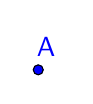
\begin{tikzpicture}[scale = 2]
	\draw
	(0,0) coordinate(A)
	(0.05,0.025) coordinate(pos)
	node[blue, anchor = south] {$\mathsf{A}$}  
	[blue,fill](A) circle(0.85pt); 
	\draw      [color = black](A) circle(0.9pt);
	\end{tikzpicture}
}
\newcommand{\Linustrik}{%  Strik, segment
	
\begin{tikzpicture}[scale = 0.4]
	\draw
	(0,0) coordinate(A)
	(1,0.7) coordinate(B)
	[line width = 1pt, blue](A)--(B);
	\draw[blue, fill](A) circle(4pt);
	\draw[blue, fill](B) circle(4pt);
	\end{tikzpicture}	
}

\newcommand{\Lina}{% bein lína, hægt að framlengja að vild
	
\begin{tikzpicture}[scale = 0.5]
	\draw
	(0,0) coordinate(A)
	(1,0.7) coordinate(B)
	[line width = 1pt, blue](A)--(B);
	\draw[blue, fill](0.25,0.18) circle(3pt);
	\draw[blue, fill](0.74,0.53) circle(3pt);
	\end{tikzpicture}	
}
\newcommand{\Halflina}{% við smíð á hornum
	
\begin{tikzpicture}[scale = 0.4]
	\draw
	(0,0) coordinate(A)
	(1,0.7) coordinate(B)
	[line width = 1pt, blue](A)--(B);
	\draw[blue, fill](A) circle(3pt);
	\draw[blue, fill](0.65,0.45) circle(3pt);
	\end{tikzpicture}	
	
}

\newcommand{\GeoO}{
	\begin{tikzpicture}[rotate=30,transform canvas={scale=0.18},yshift=7mm]
	\def\xrad{0.7}
	\def\yrad{0.58}
	\definecolor{GeogebraLitur}{rgb}{0.6,0.60,100}
	\tikzset{hnutur/.style={shape=circle, line width=0.7mm,color=black, fill=GeogebraLitur, scale=0.8, draw}} % 0.8
	\draw[ color = gray!70!black, line width=1.3mm] (0,0) circle[x radius = \xrad cm, y radius = \yrad cm];
	\def\n{5}
	\foreach \k in {1,...,\n}
	\node at ({360/\n*\k-10}:\xrad cm and \yrad cm)[hnutur] {};
	%	node[pos=1,hnutur]{} ;
	\end{tikzpicture}
}
\newcommand{\Geogebra}{{\color{gray!70!black}\textsf{Ge}\ \GeoO\textsf{Gebra }}}




% ---------- Skrá fyrir myndir ---------- 
\graphicspath{{graphics/}{Graphics/}{./}}
% ---------- Skrá fyrir heimildir ---------- 
\usepackage[style=ieee]{biblatex}
\addbibresource{bibliography.bib}
\usepackage{mathtools}
\begin{document}

%% --- Titil síða / Title page --- %%
\begin{titlepage}
	\centering
	
\includegraphics[width=0.3\textwidth]{LOGO.PNG}\par\vspace{1cm} %<-- RU Logo
	{\scshape\LARGE Indian Institute of Technology, Bombay \par} %<-- Nafn háskólans (Háskólinn í Reykjavík / Reykjavik University)
	\vspace{1cm}
	{\scshape\Large EE338 - Digital Signal Processing \par} %<-- Áfanga titill / Class or course title
	\vspace{1.5cm}
	{\huge\bfseries Digital Filter design\par} %<-- Titill Skýrslu / Title of Report
	\vspace{2cm}
	{\Large\itshape Name}\par %<-- Nafn nemanda / Name of student
	\texttt{Tejaswee Sulekh}\par %<-- t-póstfang / e-mail
	\vspace{0.7cm}
	{\Large\itshape Roll Number}\par %<-- Nafn nemanda / Name of student
	\texttt{20D070082}\par %<-- t-póstfang / e-mail
	\vfill
	Reviewed by\par %<-- (Umsjón höfðu / supervised by)
	   Hemant Hajare, 20D070037 %<-- Nafn kennara og aðstoðarkennara í tilraun / Name of Lab Teacher and TA
	\vfill

% Bottom of the page
	{\large Group Number-26\par}
\end{titlepage}

%% --- Titil síða endar / Title page ends --- %%

\section{Filter Design (BandPass)} %<--  Inngangur / Introduction

Designed a Chebyshev filter for the given specs. Calculations and detailed step-wise description is given below.

\subsection{Un-normalized discrete time filter specs}

Filter Number = 84\\
Therefore,\\
m = 4\\
q(m) = 0.1*4 = 0\\
r(m) = m - 10*q(m) = 4\\
BL(m) = 10 + 5*q(m) + 13*r(m) = 10 + 52 = 62 $Khz$\\
BH(m) = 75 + 62 = 137 $kHz$\\

Here, we have a analog signal with bandwidth of 280Khz. Where we sample it with 600Khz.

Here we have a bandpass filter with BL and BH (Khz)being the pass band frequencies for the filter to be designed. 

Hence, specifications here would be:
\begin{itemize}

\item \textbf{StopBand}: 62 to 137 Khz

\item \textbf{Transitionband}: 5Khz

\item \textbf{PassBand}: 0 to 57Khz and 142Khz to 300 Khz (As sampling frequency is 600 kHz)

\item \textbf{Tolerance}: 0.15 in magnitude for both Passband and Stopband

\item \textbf{Passband Nature}: Equiripple

\item \textbf{Stopband Nature}; Monotonic

\end{itemize}

\subsection{Normalized Digital Filter Specifications}

As we are sampling this signal at a frequency of 600 KHz. It is then normalized from 0 to   1$\pi$. By the following transformation:

\begin{equation}
    \omega = \frac{\Omega * 2 * \pi)}{\Omega_{s}(Sampling\_Rate)}
\end{equation}

Therefore the corresponding normalized discrete filter specifications are :-

\begin{itemize}

\item \textbf{PassBand}: $0.207\pi$ to $0.457\pi$

\item \textbf{Transitionband}: $0.0167\pi$

\item \textbf{StopBand}: $0 - 0.1899\pi$ to $0.4733\pi - 1\pi$

\item \textbf{Tolerance}: 0.15 in magnitude for both Passband and Stopband

\item \textbf{Passband Nature}: Equiripple

\item \textbf{Stopband Nature}; Monotonic

\end{itemize}
 
 \subsection{After applying bilinear transformation}

 The bilinear transformation is given as:

 \begin{equation}
     \Omega = tan(\frac{\omega}{2})
 \end{equation}

 \newpage

 From this transformation we end with the following new values:
\begin{table}[!h]
    \centering

\begin{tabular}{|c|c|}
\hline
Discrete & Analog \\
\hline
$0.207\pi$ & 0.3365 \\
$0.457\pi$ & 0.8723 \\
$0.0167\pi$ & 0.02618 \\
$0 - 0.1899\pi$ & 0 - 0.3076\\
$0.4733\pi - 1\pi$ & $0.9195 - \infty$ \\

\hline
\end{tabular}

\end{table}

Hence the corresponding frequencies will be as follows:

\begin{itemize}

\item \textbf{StopBand}: 0.3365 to 0.8723

\item \textbf{Transitionband}: 0.02618

\item \textbf{PassBand}: 0 to 0.3076 and 0.9195 to $\infty$

\item \textbf{Tolerance}: 0.15 in magnitude for both Passband and Stopband

\item \textbf{Passband Nature}: Equiripple

\item \textbf{Stopband Nature}; Monotonic

\end{itemize}

\subsection{Frequency Transformation and Relevant Parameters}

We need to transform the analog bandpass filter to an analog low-pass filter so that we can apply \textbf{Chebyshev} filter design on it. This is performed by using the following transformation.

\begin{equation}
    \Omega_{L} = \frac{\Omega^2 - \Omega_{o}^2}{B*\Omega}
\end{equation}

Where the two parameters above depend on the band pass frequencies in the following way:

$$\Omega_{o} = \sqrt{\Omega_{P_1}*\Omega_{P_2}} = \sqrt{0.3365 * 0.8723} = 0.5418$$
$$ B = \Omega_{P_2} - \Omega_{P_1} = 0.8723 - 0.3365 = 0.5358$$

\begin{table}[!h]
    \centering

\begin{tabular}{|c|c|}
\hline
$\Omega$ & $\Omega_L$\\
\hline
$0^+$ & $-\infty$ \\
0.3076 &  $-1.2068 (\Omega_{L_{S_1}})$\\
0.3365 & $-1 (\Omega_{L_{P_1}})$ \\
0.5418 &  $0$\\
0.8723 & $+1 (\Omega_{L_{P_2}})$\\
0.9195 & $+1.1203(\Omega_{L_{S_2}})$\\
$\infty$ & $\infty$ \\
\hline
\end{tabular}

\end{table}

\subsection{Frequency Transformed Lowpass Analog filter specification}

\begin{itemize}
    \item \textbf{Passband Edge}: $1 (\Omega_{LP})$
    \item \textbf{Stopband Edge}: $\min(\Omega_{LS1},-\Omega_{LS2}) = \min(1.2068, 1.1203) = 1.1203 (\Omega_{LS})$
    \item \textbf{Tolerance}: $0.15$ in magnitude for both Passband and Stopband
    \item \textbf{Passband Nature}: Equiripple
    \item \textbf{Stopband Nature}: Monotonic
\end{itemize}

\subsection{Analog Low pass function}
We will be using a filter which is monotonic in stopband and equiripple in passband. Therefore, we will be using \textbf{Chebyshev} filter design here for the same lets find the order for $N_{min}$ Which is shown below:

$$D_1 = \frac{1}{(1 - \delta)^2} - 1 = \frac{1}{0.85^2} - 1 = 0.3841 = \epsilon$$
$$D_2 = \frac{1}{\delta^2} - 1 = \frac{1}{0.15^2} - 1 = 43.44$$
Now using the inequality on the order N of the filter for the Chebyshev Approximation we get :-
% $$N_{min} = \left\lceil\frac{\log\sqrt{\frac{D_2}{D_1}}}{\log\frac{\Omega_S}
% {\Omega_P}}\right\rceil$$
% $$N_{min} = \left\lceil11.13\right\rceil = 12$$
$$N_{MIN} = \left\lceil\frac{Cosh^{-1}(\sqrt{\frac{D_2}{D_1}})}{Cosh^{-1}(\frac{\Omega_{L_S}}{\Omega_{L_P}})}\right\rceil$$

$$N_{MIN} = \left\lceil 6.2896 \right\rceil = 7$$

Now, the poles of the transfer function can be obtained by solving the equation :-
\begin{equation}
    \centering
1 + D_1*cosh^2(N_{MIN}*cosh^{-1}(\frac{s}{j})) = 1 + 0.3841*cosh^2(N_{MIN}*cosh^{-1}(\frac{s}{j}))
\end{equation}

After solving this equation and plotting the solutions which will give us crutial information to design the equivalent lowpass filter:

\begin{center}
    
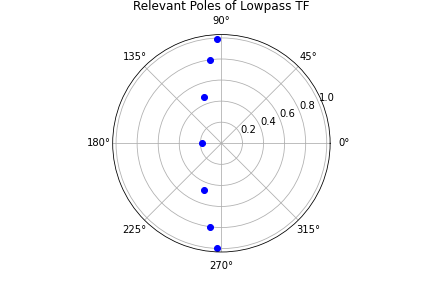
\includegraphics[width=0.6\textwidth]{Graphics/poles_lp.png}\par\vspace{2cm}

\end{center}

Where the poles are given below:

\begin{center}
$P_1 = -0.04014613-9.90667614e-01j,$\\
$P_2 = -0.11248696-7.94453744e-01j,$\\
$P_3 = -0.16254837-4.40888566e-01j,$\\
$P_4 = -0.18041508-1.86662712e-16j,$\\
$P_5 = -0.16254837+4.40888566e-01j,$\\
$P_6 = -0.11248696+7.94453744e-01j,$\\
$P_7 = -0.04014613+9.90667614e-01j,$\\ 
\end{center}

\newpage

Using the fact that we are making a Chebyschev filter with N being odd we can generate an analog lowpass filter as follows:

\begin{center}
$H_{analog},LPF (s_L) = \frac{P_1*P_2*P_3*P_4*P_5*P_6*P_7}
{(s_L - p_1)*(s_L - p_2)*(s_L - p_3)*(s_L - p_4)*(s_L - p_5)*(s_L - p_6)*(s_L - p_7)}$
\end{center}


\begin{center}
$s^{7} + 0.810777997856917 s^{6} + 7.7715611723761 \cdot 10^{-16} i s^{6} + 2.07868048090444s^{5} +$ 
\\
$6.10622663543836 \cdot 10^{-16} i s^{5} + 1.22951558147444 s^{4} +$\\
$1.22124532708767 \cdot 10^{-15} is^{4} + 1.24265791063518 s^{3} + 6.38378239159465 \cdot 10^{-16} i s^{3} + 0.461709176442476s^{2} + 4.96130914129367 \cdot 10^{-16} i s^{2} +$\\
$0.18773418093357 s + 1.66533453693773 \cdot 10^{-16} is + 0.0252120092621757 + 3.46944695195361 \cdot 10^{-17} i$
\end{center}

\subsection{Analog Bandstop Transfer Function}

This analog lowpass filter is then further transformed to the expected bandpass filter by using this following transformation:

$$sL = \frac{\Omega_{o}^2 + s^2}{B*s}$$

where B and $\Omega_{o}$ are 0.5358 and  0.5418 respectively. So after making the substitution we get:

\begin{equation}
    sL = \frac{0.5418^2 + s^2}{0.5358*s}
\end{equation}

After the transformation we get the following expression:

Where numerator is as follows ;-

\begin{center}

$- 0.0252120092621757 s^{7} - 3.62123525610158 \cdot 10^{-17} i s^{7}$

\end{center}

And the denominator is as follows :-

\begin{center}

$    78.8635872199675 s^{14} + 34.2606912621993 s^{13} + 3.90798504668055 \cdot 10^{-14} i s^{13} + 209.134616451171 s^{12} $
$+ 1.59872115546023 \cdot 10^{-14} i s^{12} + 75.2659234429593 s^{11} + 9.32587340685131 \cdot 10^{-14} i s^{11} + 219.905973975976 s^{10} + $\\
$2.8421709430404 \cdot 10^{-14} i s^{10} + 63.418346134619 s^{9} + 8.01581023779363 \cdot 10^{-14} i s^{9} + 117.873265787452 s^{8} + 1.64313007644523 \cdot 10^{-14} i s^{8} +$\\
$26.021537553505 s^{7} + 3.24740234702858 \cdot 10^{-14} i s^{7} + 34.6052445714144 s^{6} + 5.38458166943201 \cdot 10^{-15} i s^{6} + 5.46598109734443 s^{5} + $\\
$4.96477858824562 \cdot 10^{-15} i s^{5} + 5.56438085570544 s^{4} + 5.55111512312578 \cdot 10^{-16} i s^{4} + 0.559119734551591 s^{3}$\\
$+ 4.9960036108132 \cdot 10^{-16} i s^{3} + 0.456098829625325 s^{2} + 3.12250225675825 \cdot 10^{-17} i s^{2} + $\\
$0.0219359153546601 s + 2.08166817117217 \cdot 10^{-17} i s + 0.0148239101752235$
    
\end{center}

\subsection{Discrete time transfer function}

To transform the analog domain transfer function into the discrete domain, we need to make use of the Bilinear Transformation which is given as:

$$s = \frac{1 - z^{-1}}{1 + z^{-1}}$$

after the conversion we get the following results:
\newpage

Where numerator and denominator are shown below:

Numerator:
\begin{center}
    $0.0252120092621757 \left(z^{-1}\right)^{21} + 3.62123525610158 \cdot 10^{-17} i \left(z^{-1}\right)^{21} $\\ 
    $+ 0.17648406483523 \left(z^{-1}\right)^{20} + 2.53486467927111 \cdot 10^{-16} i \left(z^{-1}\right)^{20} + 0.35296812967046 \left(z^{-1}\right)^{19} $\\
    $+ 5.06972935854222 \cdot 10^{-16} i \left(z^{-1}\right)^{19} - 0.35296812967046 \left(z^{-1}\right)^{18} -$\\
    $ 5.06972935854222 \cdot 10^{-16} i \left(z^{-1}\right)^{18} - 2.29429284285799 \left(z^{-1}\right)^{17} - $\\ 
    $3.29532408305244 \cdot 10^{-15} i \left(z^{-1}\right)^{17} - 1.94132471318753 \left(z^{-1}\right)^{16} - $\\ 
    $2.78835114719822 \cdot 10^{-15} i \left(z^{-1}\right)^{16} + 4.23561755604552 \left(z^{-1}\right)^{15} + $\\ 
    $6.08367523025066 \cdot 10^{-15} i \left(z^{-1}\right)^{15} + 8.67293118618846 \left(z^{-1}\right)^{14} + $\\ 
    $1.24570492809895 \cdot 10^{-14} i \left(z^{-1}\right)^{14} - 0.35296812967046 \left(z^{-1}\right)^{13} - $\\ 
    $5.06972935854222 \cdot 10^{-16} i \left(z^{-1}\right)^{13} - 13.765757057148 \left(z^{-1}\right)^{12} - $\\ 
    $1.97719444983147 \cdot 10^{-14} i \left(z^{-1}\right)^{12} - 9.17717137143197 \left(z^{-1}\right)^{11} - $\\ 
    $1.31812963322098 \cdot 10^{-14} i \left(z^{-1}\right)^{11} + 9.17717137143197 \left(z^{-1}\right)^{10} +$\\ 
    $ 1.31812963322098 \cdot 10^{-14} i \left(z^{-1}\right)^{10} + 13.765757057148 \left(z^{-1}\right)^{9} + $\\ 
    $1.97719444983147 \cdot 10^{-14} i \left(z^{-1}\right)^{9} + 0.35296812967046 \left(z^{-1}\right)^{8} + $\\ 
    $5.06972935854222 \cdot 10^{-16} i \left(z^{-1}\right)^{8} - 8.67293118618846 \left(z^{-1}\right)^{7} - $\\ 
    $1.24570492809895 \cdot 10^{-14} i \left(z^{-1}\right)^{7} - $\\ 
    $4.23561755604552 \left(z^{-1}\right)^{6} - 6.08367523025066 \cdot 10^{-15} i \left(z^{-1}\right)^{6} + 1.94132471318753 \left(z^{-1}\right)^{5} + $\\
    $2.78835114719822 \cdot 10^{-15} i \left(z^{-1}\right)^{5} + 2.29429284285799 \left(z^{-1}\right)^{4} + $\\ 
    $3.29532408305244 \cdot 10^{-15} i \left(z^{-1}\right)^{4} + 0.35296812967046 \left(z^{-1}\right)^{3} + $\\ 
    $5.06972935854222 \cdot 10^{-16} i \left(z^{-1}\right)^{3} - 0.35296812967046 \left(z^{-1}\right)^{2} -$\\ 
    $ 5.06972935854222 \cdot 10^{-16} i \left(z^{-1}\right)^{2} - $\\ 
    $0.17648406483523 z^{-1} - 2.53486467927111 \cdot 10^{-16} i z^{-1} - $\\ 
    $0.0252120092621757 - 3.62123525610158 \cdot 10^{-17} i$
\end{center}


Denominator:

\begin{center}

    $461.404456460953 \left(z^{-1}\right)^{21} - 1.61049500889819 \cdot 10^{-13} i \left(z^{-1}\right)^{21}$ \\ 
    $ - 173.093314501077 \left(z^{-1}\right)^{20} - 9.66427651872398 \cdot 10^{-14} i \left(z^{-1}\right)^{20}$ \\ 
    $ - 233.590871479053 \left(z^{-1}\right)^{19} + 2.37643930876021 \cdot 10^{-13} i \left(z^{-1}\right)^{19}$ \\ 
    $ + 2842.27305876781 \left(z^{-1}\right)^{18} - 6.71492194688749 \cdot 10^{-13} i \left(z^{-1}\right)^{18}$ \\ 
    $ - 1212.41127249349 \left(z^{-1}\right)^{17} - 5.6614624374733 \cdot 10^{-13} i \left(z^{-1}\right)^{17}$ \\ 
    $ - 803.497825995003 \left(z^{-1}\right)^{16} + 1.10746542027395 \cdot 10^{-12} i \left(z^{-1}\right)^{16}$ \\ 
    $ + 8046.32066101662 \left(z^{-1}\right)^{15} - 1.33056176914832 \cdot 10^{-12} i \left(z^{-1}\right)^{15} - $ \\ 
    $3728.11909618479 \left(z^{-1}\right)^{14} - 1.55936233397121 \cdot 10^{-12} i \left(z^{-1}\right)^{14}$ \\ 
    $ - 934.538053613733 \left(z^{-1}\right)^{13} + 2.54753696510892 \cdot 10^{-12} i \left(z^{-1}\right)^{13}$ \\ 
    $ + 13394.697419938 \left(z^{-1}\right)^{12} - 1.4107453386545 \cdot 10^{-12} i \left(z^{-1}\right)^{12}$ \\ 
    $ - 6344.79529753947 \left(z^{-1}\right)^{11} - 2.55766267418136 \cdot 10^{-12} i \left(z^{-1}\right)^{11}$ \\ 
    $ - 19.6396526241181 \left(z^{-1}\right)^{10} + 3.50060734313685 \cdot 10^{-12} i \left(z^{-1}\right)^{10}$ \\ 
    $ + 14177.8498324867 \left(z^{-1}\right)^{9} - 5.80655286940461 \cdot 10^{-13} i \left(z^{-1}\right)^{9}$ \\ 
    $ - 6353.9923950893 \left(z^{-1}\right)^{8} - 2.59427508548964 \cdot 10^{-12} i \left(z^{-1}\right)^{8}$ \\ 
    $ + 911.649579424513 \left(z^{-1}\right)^{7} + 2.9746892803304 \cdot 10^{-12} i \left(z^{-1}\right)^{7}$ \\ 
    $ + 9682.84755463498 \left(z^{-1}\right)^{6} + 3.8615526756652 \cdot 10^{-13} i \left(z^{-1}\right)^{6}$ \\ 
    $ - 3623.87908365985 \left(z^{-1}\right)^{5} - 1.56761471102799 \cdot 10^{-12} i \left(z^{-1}\right)^{5}$ \\ 
    $ + 797.256090809802 \left(z^{-1}\right)^{4} + 1.48874295109102 \cdot 10^{-12} i \left(z^{-1}\right)^{4}$ \\ 
    $ + 4079.54821578256 \left(z^{-1}\right)^{3} + 6.2969514488262 \cdot 10^{-13} i \left(z^{-1}\right)^{3}$ \\ 
    $ - 966.166930603176 \left(z^{-1}\right)^{2} - 4.70568122138398 \cdot 10^{-13} i \left(z^{-1}\right)^{2}$ \\ 
    $ + 216.438269509398 z^{-1} + 3.40442212921652 \cdot 10^{-13} i z^{-1} + 871.43152674202$ \\ 
    $ + 2.86432206245709 \cdot 10^{-13} i$
    
\end{center}

\newpage


\section{Results and Discussion} 

\subsection{Analog Lowpass Filter}

After obtaining the poles for analog relevant lowpass filter we get the following amplitude response plot. Where we can clearly see that the specifications are met.
\vspace{0.5cm}
\begin{center}
    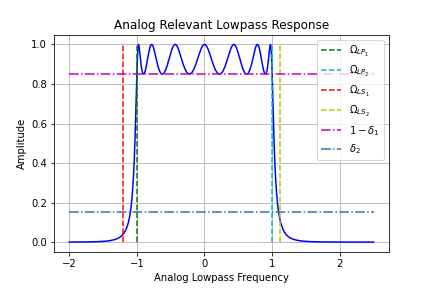
\includegraphics[width=0.6\textwidth]{Graphics/Lowpass.png}\par\vspace{0.5cm}    
\end{center}
\begin{center}
    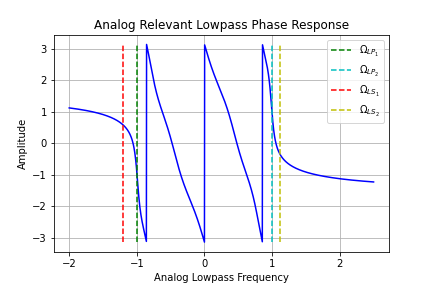
\includegraphics[width=0.6\textwidth]{Graphics/LpPhase.png}\par\vspace{0.2cm}    
\end{center}

\newpage

\subsection{Analog Bandpass Filter}

As we obtain the relevant low-pass filter after applying the corresponding transformations. We get the following poles and magnitude response.
\vspace{1cm}
\begin{center}
    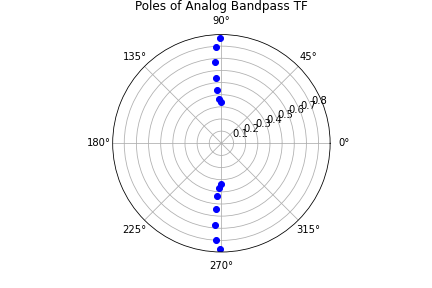
\includegraphics[width=0.6\textwidth]{Graphics/Poles_bp.png}\par\vspace{0.2cm}
\end{center}

\begin{center}
    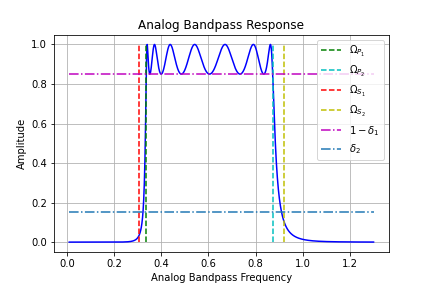
\includegraphics[width=0.6\textwidth]{Graphics/Bandpass.png}\par\vspace{0.2cm}
\end{center}

\begin{center}
    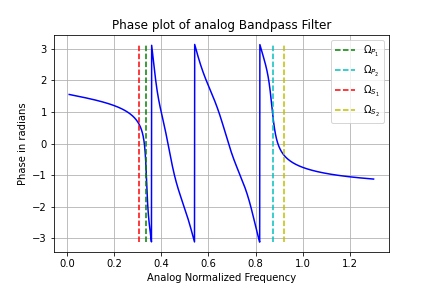
\includegraphics[width=0.6\textwidth]{Graphics/PhaseBP.png}\par\vspace{0.2cm}
\end{center}

Again we observe that the values for passband and stopband matched the calculated ones and our filter has the required tolerances and equiripples nature.

\subsection{Coming Back to Discrete Domain}

Then finally we apply Bilinear transformation to come back to discrete domain in which we are trying to meet the specifications. After this we get the following plots.


\begin{center}
    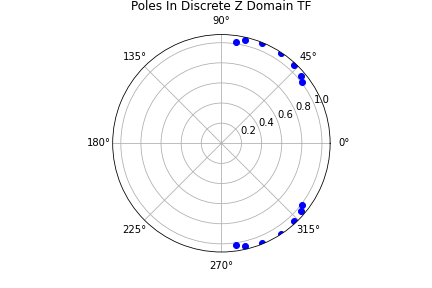
\includegraphics[width=0.6\textwidth]{Graphics/Poles_z.png}\par\vspace{0.2cm}
\end{center}

\begin{center}
    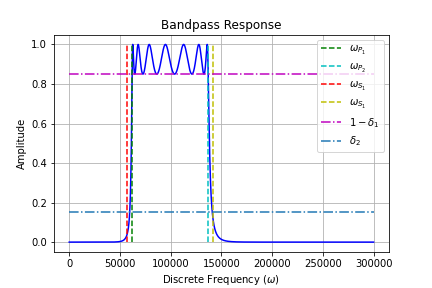
\includegraphics[width=0.6\textwidth]{Graphics/Zreal.png}\par\vspace{0.2cm}
\end{center}
\begin{center}
    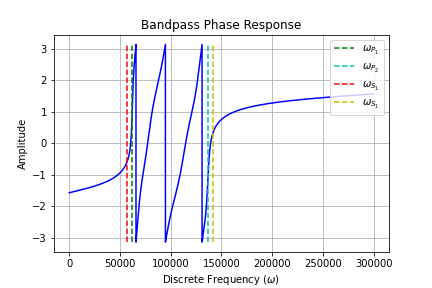
\includegraphics[width=0.6\textwidth]{Graphics/Zphase.png}\par\vspace{0.2cm}    
\end{center}

Filter that we designed meets the specifications and tolerance requirements as can be seen below.\\

I've reviewed my teammate's report Samriddhi Mishra (20D070068). She followed the same methodology as done in previous years resources. Her plots were clear and came out correctly only. Since she designed bandstop filter reviewing her phase plots was a bit difficult.

\end{document}
